\section{Acceleration limit and voltage-step response}

\subsection*{Q5 -- Maximum acceleration before mass--waveguide contact}

An acceleration $a$ along the motion axis loads every suspended part with a
body force $\rho a$ per unit volume. Contact occurs when the modulation bar
crosses the \SI{200}{\nano\meter} gap to the waveguide, $u_{y}=+g_{0}$. For
each bias the model is solved at two accelerations, $a_{\max}$ follows from
linear scaling, and a third solve at $a_{\max}$ verifies the result; the
verification residuals stay below 0.2\%, so the linear treatment is justified.
Table~\ref{tab:q5} and Fig.~\ref{fig:q5} give the results.

\begin{table}[H]
\centering
\small
\caption{Maximum tolerable DC acceleration toward the waveguide.}
\label{tab:q5}
\begin{tabular}{cccc}
\toprule
$\Vd$ & rest position $u_{y}$ & $a_{\max}$ (\si{\meter\per\second\squared}) & in $g$\\
\midrule
\SI{0}{\volt}  & 0                       & $1.903\times10^{6}$ & 193\,950\\
\SI{1}{\volt}  & \SI{-0.002}{\nano\meter} & $1.903\times10^{6}$ & 193\,950\\
\SI{10}{\volt} & \SI{-0.160}{\nano\meter} & $1.904\times10^{6}$ & 194\,060\\
\SI{50}{\volt} & \SI{-4.03}{\nano\meter}  & $1.930\times10^{6}$ & 196\,690\\
\bottomrule
\end{tabular}
\end{table}

\begin{figure}[H]
\centering
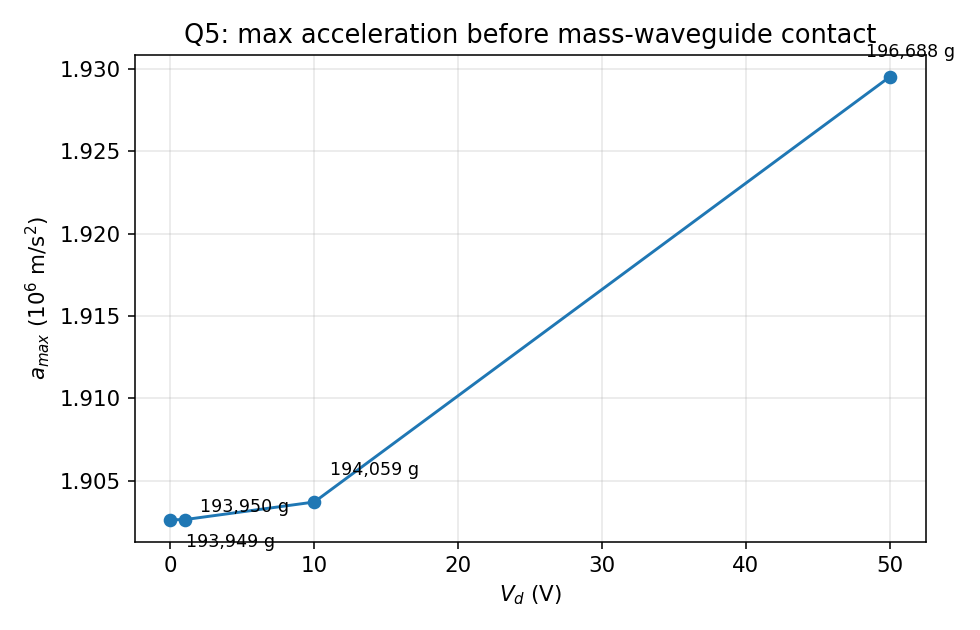
\includegraphics[width=0.66\textwidth]{figures/q5_max_acceleration.png}
\caption{Maximum acceleration versus bias voltage. The bias moves the shuttle
away from the waveguide, so the tolerance grows slightly with $\Vd$.}
\label{fig:q5}
\end{figure}

The bias dependence is weak but has a definite sign: $a_{\max}$
\emph{increases} with $\Vd$, by 1.4\% at \SI{50}{\volt}. The comb pulls the
shuttle away from the waveguide, which adds travel margin, and the tip-gap
attraction weakens as the shuttle moves up, which helps further. Part~1
assumed the opposite sign (bias displacement toward the waveguide) and should
be corrected on this point in the final report.

The magnitude also differs from Part~1's $3.46\times10^{6}~\si{\meter\per\second\squared}$.
Dividing $kg_{0}$ by the FEM limit gives an effective inertia of
\SI{3.88}{\pico\gram}: the figure-true shuttle plus about half the beam mass,
since the distributed body load also bends the beams directly. Part~1's
smaller mass (\SI{2.33}{\pico\gram}) and stiffer spring account for the rest.
Either way, the static shock tolerance is around $2\times10^{5}\,g$; as in
Part~1, the practical concern is excitation near resonance, not static
acceleration.

\subsection*{Q6 -- Voltage-step response, 1 V and 50 V}

The drive electrode receives a smoothed voltage step (rise time
\SI{1}{\micro\second}, well below the \SI{2}{\micro\second} oscillation
period but gentle enough for the coupled solid--electrostatics--moving-mesh
integrator, which fails on nanosecond-scale steps). Rayleigh damping is the
same as in Q3. Figure~\ref{fig:q6resp} shows both responses;
Fig.~\ref{fig:q6norm} overlays them with the Q3 force step, normalised to
their final values.

\begin{figure}[H]
\centering
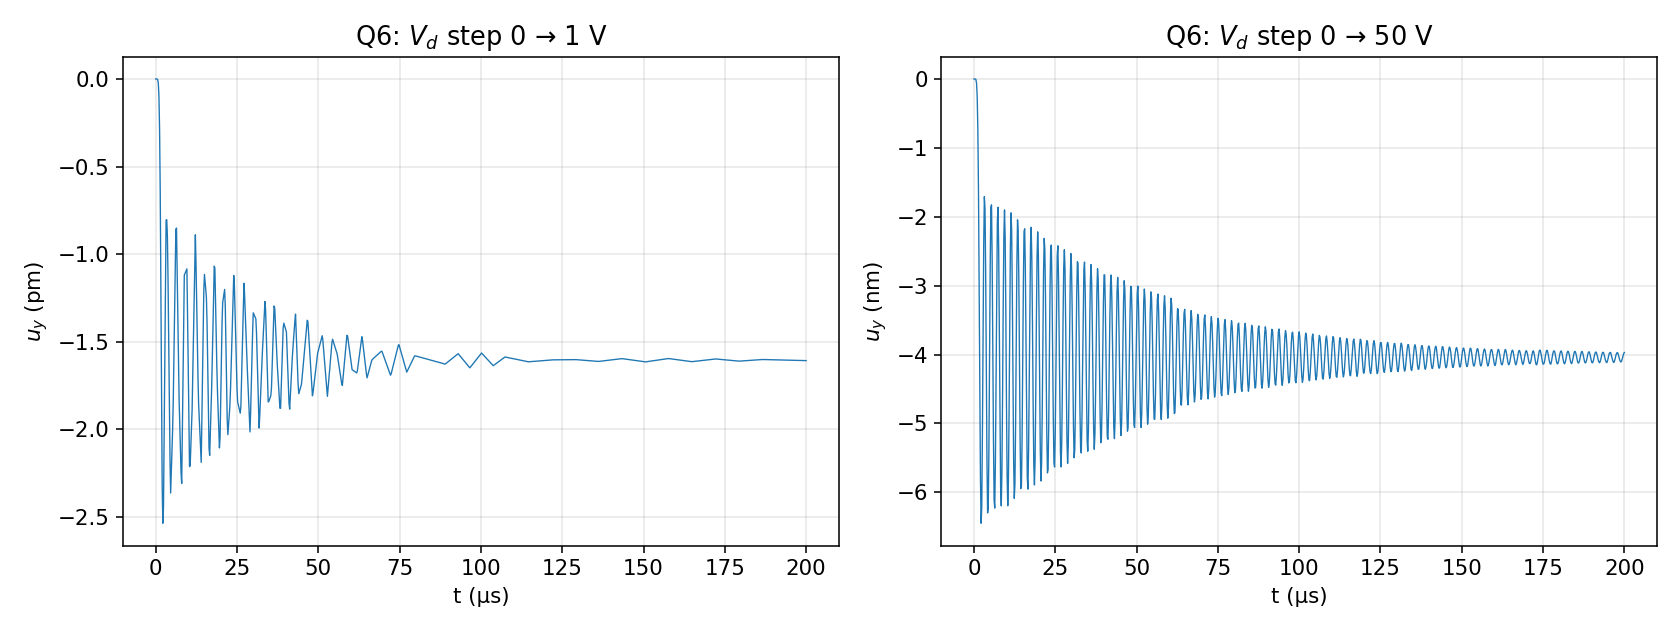
\includegraphics[width=\textwidth]{figures/q6_vstep_responses.png}
\caption{Step responses for $\Vd$: $0\to\SI{1}{\volt}$ (left, picometre
scale) and $0\to\SI{50}{\volt}$ (right, nanometre scale). Note the $2500:1$
amplitude ratio for a $50:1$ voltage ratio.}
\label{fig:q6resp}
\end{figure}

\begin{figure}[H]
\centering

\includegraphics[width=0.8\textwidth]{figures/q6_vs_q3_normalized.png}
\caption{Normalised comparison of the Q3 force step and the Q6 voltage
steps. All three ring at $f_{1}$ and settle on the same time scale; the
voltage steps overshoot less because of the \SI{1}{\micro\second} input
rise.}
\label{fig:q6norm}
\end{figure}

The comparison with Q3 comes down to three observations.

First, the dynamics are identical. Both responses ring at
$f_{1}=\SI{496}{\kilo\hertz}$ and the \SI{50}{\volt} step settles in about
\SI{150}{\micro\second}, matching Q3's \SI{158}{\micro\second} within the
numerical accuracy of the coupled transient. At these voltages the device
operates far below pull-in (\SI{222}{\volt}), so the electromechanical system
is effectively linear and a voltage step acts exactly like a force step of
size $F=\tfrac{1}{2}V^{2}\,dC/dx$. The bias softening measured in Q4b
supports this: at \SI{50}{\volt} the mode-1 frequency shifts by only $-0.3$\%,
invisible in the ringing.

Second, the input scaling is quadratic, and that is the real difference
between the two experiments. Final values are \SI{-1.61}{\pico\meter} at
\SI{1}{\volt} and \SI{-3.97}{\nano\meter} at \SI{50}{\volt} -- a factor 2466
for a factor 50 in voltage, against 2500 expected from $V^{2}$ (the static
values from Q4a are reproduced to within 1.7\%). A force input scales
linearly; a voltage input does not. For the phase-shifter application this
is the linearity limit of the actuator, independent of any mechanical
nonlinearity.

Third, the overshoot is $1.62\times$ instead of Q3's $1.96\times$. This is
the input, not the plant: the \SI{1}{\micro\second} rise filters the step.
The same filtering appears identically in both Q6 traces.

One numerical remark. The \SI{50}{\volt} trace is quantitative (envelope
decay within 7\% of $\zeta\omega_{1}$). The \SI{1}{\volt} response, at
\SI{1.6}{\pico\meter}, sits below the integrator's effective absolute error
floor, and its apparent decay is dominated by numerical dissipation even at a
relative tolerance of $10^{-5}$ -- re-running with tighter settings did not
change it. The waveform and final value are correct; the decay is not. Since
the system is linear at these amplitudes, the physical \SI{1}{\volt}
transient is the \SI{50}{\volt} trace scaled by $1/2500$, with the same
settling time. Resolving picometre transients directly would need manual
per-variable absolute tolerances, which is beyond what the comparison
requires.
